% Options for packages loaded elsewhere
\PassOptionsToPackage{unicode}{hyperref}
\PassOptionsToPackage{hyphens}{url}
\PassOptionsToPackage{dvipsnames,svgnames,x11names}{xcolor}
%
\documentclass[
]{report}

\usepackage{amsmath,amssymb}
\usepackage{iftex}
\ifPDFTeX
  \usepackage[T1]{fontenc}
  \usepackage[utf8]{inputenc}
  \usepackage{textcomp} % provide euro and other symbols
\else % if luatex or xetex
  \usepackage{unicode-math}
  \defaultfontfeatures{Scale=MatchLowercase}
  \defaultfontfeatures[\rmfamily]{Ligatures=TeX,Scale=1}
\fi
\usepackage[sfdefault]{roboto}
\ifPDFTeX\else  
    % xetex/luatex font selection
\fi
% Use upquote if available, for straight quotes in verbatim environments
\IfFileExists{upquote.sty}{\usepackage{upquote}}{}
\IfFileExists{microtype.sty}{% use microtype if available
  \usepackage[]{microtype}
  \UseMicrotypeSet[protrusion]{basicmath} % disable protrusion for tt fonts
}{}
\makeatletter
\@ifundefined{KOMAClassName}{% if non-KOMA class
  \IfFileExists{parskip.sty}{%
    \usepackage{parskip}
  }{% else
    \setlength{\parindent}{0pt}
    \setlength{\parskip}{6pt plus 2pt minus 1pt}}
}{% if KOMA class
  \KOMAoptions{parskip=half}}
\makeatother
\usepackage{xcolor}
\usepackage[margin=1in]{geometry}
\setlength{\emergencystretch}{3em} % prevent overfull lines
\setcounter{secnumdepth}{-\maxdimen} % remove section numbering
% Make \paragraph and \subparagraph free-standing
\makeatletter
\ifx\paragraph\undefined\else
  \let\oldparagraph\paragraph
  \renewcommand{\paragraph}{
    \@ifstar
      \xxxParagraphStar
      \xxxParagraphNoStar
  }
  \newcommand{\xxxParagraphStar}[1]{\oldparagraph*{#1}\mbox{}}
  \newcommand{\xxxParagraphNoStar}[1]{\oldparagraph{#1}\mbox{}}
\fi
\ifx\subparagraph\undefined\else
  \let\oldsubparagraph\subparagraph
  \renewcommand{\subparagraph}{
    \@ifstar
      \xxxSubParagraphStar
      \xxxSubParagraphNoStar
  }
  \newcommand{\xxxSubParagraphStar}[1]{\oldsubparagraph*{#1}\mbox{}}
  \newcommand{\xxxSubParagraphNoStar}[1]{\oldsubparagraph{#1}\mbox{}}
\fi
\makeatother

\usepackage{color}
\usepackage{fancyvrb}
\newcommand{\VerbBar}{|}
\newcommand{\VERB}{\Verb[commandchars=\\\{\}]}
\DefineVerbatimEnvironment{Highlighting}{Verbatim}{commandchars=\\\{\}}
% Add ',fontsize=\small' for more characters per line
\usepackage{framed}
\definecolor{shadecolor}{RGB}{241,243,245}
\newenvironment{Shaded}{\begin{snugshade}}{\end{snugshade}}
\newcommand{\AlertTok}[1]{\textcolor[rgb]{0.68,0.00,0.00}{#1}}
\newcommand{\AnnotationTok}[1]{\textcolor[rgb]{0.37,0.37,0.37}{#1}}
\newcommand{\AttributeTok}[1]{\textcolor[rgb]{0.40,0.45,0.13}{#1}}
\newcommand{\BaseNTok}[1]{\textcolor[rgb]{0.68,0.00,0.00}{#1}}
\newcommand{\BuiltInTok}[1]{\textcolor[rgb]{0.00,0.23,0.31}{#1}}
\newcommand{\CharTok}[1]{\textcolor[rgb]{0.13,0.47,0.30}{#1}}
\newcommand{\CommentTok}[1]{\textcolor[rgb]{0.37,0.37,0.37}{#1}}
\newcommand{\CommentVarTok}[1]{\textcolor[rgb]{0.37,0.37,0.37}{\textit{#1}}}
\newcommand{\ConstantTok}[1]{\textcolor[rgb]{0.56,0.35,0.01}{#1}}
\newcommand{\ControlFlowTok}[1]{\textcolor[rgb]{0.00,0.23,0.31}{\textbf{#1}}}
\newcommand{\DataTypeTok}[1]{\textcolor[rgb]{0.68,0.00,0.00}{#1}}
\newcommand{\DecValTok}[1]{\textcolor[rgb]{0.68,0.00,0.00}{#1}}
\newcommand{\DocumentationTok}[1]{\textcolor[rgb]{0.37,0.37,0.37}{\textit{#1}}}
\newcommand{\ErrorTok}[1]{\textcolor[rgb]{0.68,0.00,0.00}{#1}}
\newcommand{\ExtensionTok}[1]{\textcolor[rgb]{0.00,0.23,0.31}{#1}}
\newcommand{\FloatTok}[1]{\textcolor[rgb]{0.68,0.00,0.00}{#1}}
\newcommand{\FunctionTok}[1]{\textcolor[rgb]{0.28,0.35,0.67}{#1}}
\newcommand{\ImportTok}[1]{\textcolor[rgb]{0.00,0.46,0.62}{#1}}
\newcommand{\InformationTok}[1]{\textcolor[rgb]{0.37,0.37,0.37}{#1}}
\newcommand{\KeywordTok}[1]{\textcolor[rgb]{0.00,0.23,0.31}{\textbf{#1}}}
\newcommand{\NormalTok}[1]{\textcolor[rgb]{0.00,0.23,0.31}{#1}}
\newcommand{\OperatorTok}[1]{\textcolor[rgb]{0.37,0.37,0.37}{#1}}
\newcommand{\OtherTok}[1]{\textcolor[rgb]{0.00,0.23,0.31}{#1}}
\newcommand{\PreprocessorTok}[1]{\textcolor[rgb]{0.68,0.00,0.00}{#1}}
\newcommand{\RegionMarkerTok}[1]{\textcolor[rgb]{0.00,0.23,0.31}{#1}}
\newcommand{\SpecialCharTok}[1]{\textcolor[rgb]{0.37,0.37,0.37}{#1}}
\newcommand{\SpecialStringTok}[1]{\textcolor[rgb]{0.13,0.47,0.30}{#1}}
\newcommand{\StringTok}[1]{\textcolor[rgb]{0.13,0.47,0.30}{#1}}
\newcommand{\VariableTok}[1]{\textcolor[rgb]{0.07,0.07,0.07}{#1}}
\newcommand{\VerbatimStringTok}[1]{\textcolor[rgb]{0.13,0.47,0.30}{#1}}
\newcommand{\WarningTok}[1]{\textcolor[rgb]{0.37,0.37,0.37}{\textit{#1}}}

\providecommand{\tightlist}{%
  \setlength{\itemsep}{0pt}\setlength{\parskip}{0pt}}\usepackage{longtable,booktabs,array}
\usepackage{calc} % for calculating minipage widths
% Correct order of tables after \paragraph or \subparagraph
\usepackage{etoolbox}
\makeatletter
\patchcmd\longtable{\par}{\if@noskipsec\mbox{}\fi\par}{}{}
\makeatother
% Allow footnotes in longtable head/foot
\IfFileExists{footnotehyper.sty}{\usepackage{footnotehyper}}{\usepackage{footnote}}
\makesavenoteenv{longtable}
\usepackage{graphicx}
\makeatletter
\newsavebox\pandoc@box
\newcommand*\pandocbounded[1]{% scales image to fit in text height/width
  \sbox\pandoc@box{#1}%
  \Gscale@div\@tempa{\textheight}{\dimexpr\ht\pandoc@box+\dp\pandoc@box\relax}%
  \Gscale@div\@tempb{\linewidth}{\wd\pandoc@box}%
  \ifdim\@tempb\p@<\@tempa\p@\let\@tempa\@tempb\fi% select the smaller of both
  \ifdim\@tempa\p@<\p@\scalebox{\@tempa}{\usebox\pandoc@box}%
  \else\usebox{\pandoc@box}%
  \fi%
}
% Set default figure placement to htbp
\def\fps@figure{htbp}
\makeatother

\usepackage{fvextra}
\DefineVerbatimEnvironment{Highlighting}{Verbatim}{breaklines,commandchars=\\\{\}}
\makeatletter
\@ifpackageloaded{tcolorbox}{}{\usepackage[skins,breakable]{tcolorbox}}
\@ifpackageloaded{fontawesome5}{}{\usepackage{fontawesome5}}
\definecolor{quarto-callout-color}{HTML}{909090}
\definecolor{quarto-callout-note-color}{HTML}{0758E5}
\definecolor{quarto-callout-important-color}{HTML}{CC1914}
\definecolor{quarto-callout-warning-color}{HTML}{EB9113}
\definecolor{quarto-callout-tip-color}{HTML}{00A047}
\definecolor{quarto-callout-caution-color}{HTML}{FC5300}
\definecolor{quarto-callout-color-frame}{HTML}{acacac}
\definecolor{quarto-callout-note-color-frame}{HTML}{4582ec}
\definecolor{quarto-callout-important-color-frame}{HTML}{d9534f}
\definecolor{quarto-callout-warning-color-frame}{HTML}{f0ad4e}
\definecolor{quarto-callout-tip-color-frame}{HTML}{02b875}
\definecolor{quarto-callout-caution-color-frame}{HTML}{fd7e14}
\makeatother
\makeatletter
\@ifpackageloaded{caption}{}{\usepackage{caption}}
\AtBeginDocument{%
\ifdefined\contentsname
  \renewcommand*\contentsname{Table of contents}
\else
  \newcommand\contentsname{Table of contents}
\fi
\ifdefined\listfigurename
  \renewcommand*\listfigurename{List of Figures}
\else
  \newcommand\listfigurename{List of Figures}
\fi
\ifdefined\listtablename
  \renewcommand*\listtablename{List of Tables}
\else
  \newcommand\listtablename{List of Tables}
\fi
\ifdefined\figurename
  \renewcommand*\figurename{Figure}
\else
  \newcommand\figurename{Figure}
\fi
\ifdefined\tablename
  \renewcommand*\tablename{Table}
\else
  \newcommand\tablename{Table}
\fi
}
\@ifpackageloaded{float}{}{\usepackage{float}}
\floatstyle{ruled}
\@ifundefined{c@chapter}{\newfloat{codelisting}{h}{lop}}{\newfloat{codelisting}{h}{lop}[chapter]}
\floatname{codelisting}{Listing}
\newcommand*\listoflistings{\listof{codelisting}{List of Listings}}
\makeatother
\makeatletter
\makeatother
\makeatletter
\@ifpackageloaded{caption}{}{\usepackage{caption}}
\@ifpackageloaded{subcaption}{}{\usepackage{subcaption}}
\makeatother

\usepackage{bookmark}

\IfFileExists{xurl.sty}{\usepackage{xurl}}{} % add URL line breaks if available
\urlstyle{same} % disable monospaced font for URLs
\hypersetup{
  pdftitle={Tutorial III.III - DataFrames in Julia},
  colorlinks=true,
  linkcolor={blue},
  filecolor={Maroon},
  citecolor={Blue},
  urlcolor={Blue},
  pdfcreator={LaTeX via pandoc}}


\title{Tutorial III.III - DataFrames in Julia}
\usepackage{etoolbox}
\makeatletter
\providecommand{\subtitle}[1]{% add subtitle to \maketitle
  \apptocmd{\@title}{\par {\large #1 \par}}{}{}
}
\makeatother
\subtitle{Applied Optimization with Julia}
\author{}
\date{}

\begin{document}
\maketitle


\chapter{Introduction}\label{introduction}

Welcome to this tutorial on plotting in Julia! We'll be using the
powerful Plots.jl package to create beautiful and informative
visualizations. Don't worry if you're new to plotting -- we'll start
with the basics and gradually build up to more advanced techniques.

In this tutorial, you'll learn how to: 1. Create simple plots like line
graphs and scatter plots 2. Customize your plots with colors, labels,
and styles 3. Add multiple data series to a single plot 4. Save your
plots as image files for use in reports or presentations

Follow the instructions, write your code in the designated code blocks,
and validate your results with @assert statements.

Before we begin, let's make sure you have the necessary packages
installed. If you've been following the course, you'll need to install
the Plots and StatsPlots packages:

\begin{Shaded}
\begin{Highlighting}[]
\ImportTok{import} \BuiltInTok{Pkg;}\NormalTok{ Pkg.add(["Plots",}\BuiltInTok{"StatsPlots"])}
\end{Highlighting}
\end{Shaded}

Now, let's load these packages:

\begin{Shaded}
\begin{Highlighting}[]
\ImportTok{using} \BuiltInTok{Plots}\NormalTok{, }\BuiltInTok{StatsPlots}
\end{Highlighting}
\end{Shaded}

\chapter{Section 1 - Creating Basic
Plots}\label{section-1---creating-basic-plots}

The Plots.jl package simplifies the process of creating a wide array of
plots, from simple line plots to complex 3D visualizations. Let's start
with the simplest type of plot: a line plot. We'll create some example
data and then plot it.

\begin{Shaded}
\begin{Highlighting}[]
\CommentTok{\# Create some example data}
\NormalTok{x }\OperatorTok{=} \FloatTok{1}\OperatorTok{:}\FloatTok{10}      \CommentTok{\# This creates a range of numbers from 1 to 10}
\NormalTok{y }\OperatorTok{=} \FunctionTok{rand}\NormalTok{(}\FloatTok{10}\NormalTok{)  }\CommentTok{\# This creates 10 random numbers between 0 and 1}

\CommentTok{\# Create a basic line plot}
\NormalTok{line\_plot }\OperatorTok{=} \FunctionTok{plot}\NormalTok{(}
\NormalTok{    x, y, }
\NormalTok{    title}\OperatorTok{=}\StringTok{"My First Line Plot"}\NormalTok{, }
\NormalTok{    xlabel}\OperatorTok{=}\StringTok{"X{-}axis Label"}\NormalTok{, }
\NormalTok{    ylabel}\OperatorTok{=}\StringTok{"Y{-}axis Label"}\NormalTok{, }
\NormalTok{    legend}\OperatorTok{=}\ConstantTok{false}
\NormalTok{)}

\CommentTok{\# Display the plot}
\FunctionTok{display}\NormalTok{(line\_plot)}
\end{Highlighting}
\end{Shaded}

\pandocbounded{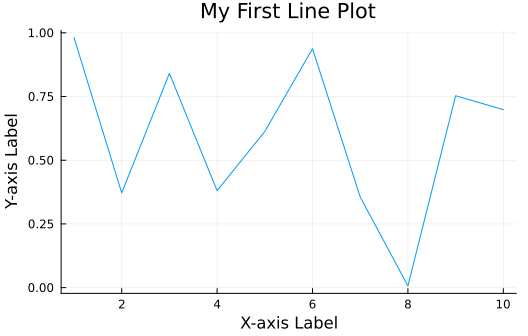
\includegraphics[keepaspectratio]{tutorial-03-05-Plotting_files/mediabag/tutorial-03-05-Plotting_files/figure-pdf/cell-4-output-1.pdf}}

Let's break down what each part of this code does:

\begin{itemize}
\tightlist
\item
  \texttt{plot(x,\ y,\ ...)} creates the plot using our x and y data
\item
  \texttt{title=...} sets the title of the plot
\item
  \texttt{xlabel=...} and \texttt{ylabel=...} label the x and y axes
\item
  \texttt{legend=false} turns off the legend (we'll use this later)
\end{itemize}

\section{Exercise 1.1 - Create a Scatter
Plot}\label{exercise-1.1---create-a-scatter-plot}

Now it's your turn! Create a scatter plot using the \texttt{scatter()}
function instead of \texttt{plot()}. Use a range from 1 to 20 for x, and
generate 20 random numbers for y.

\begin{Shaded}
\begin{Highlighting}[]
\CommentTok{\# YOUR CODE BELOW}
\CommentTok{\# Hint: Use x = 1:20 and y = rand(20)}
\end{Highlighting}
\end{Shaded}

\begin{Shaded}
\begin{Highlighting}[]
\CommentTok{\# Test your answer}
\PreprocessorTok{@assert} \PreprocessorTok{@isdefined}\NormalTok{ scatter\_plot}
\FunctionTok{println}\NormalTok{(}\StringTok{"Great job! You\textquotesingle{}ve created your first scatter plot."}\NormalTok{)}
\end{Highlighting}
\end{Shaded}

\chapter{Section 2 - Customizing
Plots}\label{section-2---customizing-plots}

One of the best things about Plots.jl is how easy it is to customize
your plots. Let's explore some options:

\begin{Shaded}
\begin{Highlighting}[]
\NormalTok{x }\OperatorTok{=} \FloatTok{1}\OperatorTok{:}\FloatTok{10}
\NormalTok{y }\OperatorTok{=} \FunctionTok{rand}\NormalTok{(}\FloatTok{10}\NormalTok{)}

\NormalTok{custom\_plot }\OperatorTok{=} \FunctionTok{plot}\NormalTok{(}
\NormalTok{    x, y,}
\NormalTok{    title}\OperatorTok{=}\StringTok{"Customized Line Plot"}\NormalTok{,}
\NormalTok{    xlabel}\OperatorTok{=}\StringTok{"X{-}axis"}\NormalTok{,}
\NormalTok{    ylabel}\OperatorTok{=}\StringTok{"Y{-}axis"}\NormalTok{,}
\NormalTok{    line}\OperatorTok{=}\NormalTok{(}\OperatorTok{:}\NormalTok{dash, }\FloatTok{2}\NormalTok{),  }\CommentTok{\# Dashed line with width 2}
\NormalTok{    color}\OperatorTok{=:}\NormalTok{red,       }\CommentTok{\# Red color}
\NormalTok{    marker}\OperatorTok{=}\NormalTok{(}\OperatorTok{:}\NormalTok{circle, }\FloatTok{8}\NormalTok{)  }\CommentTok{\# Circle markers of size 8}
\NormalTok{)}

\FunctionTok{display}\NormalTok{(custom\_plot)}
\end{Highlighting}
\end{Shaded}

\pandocbounded{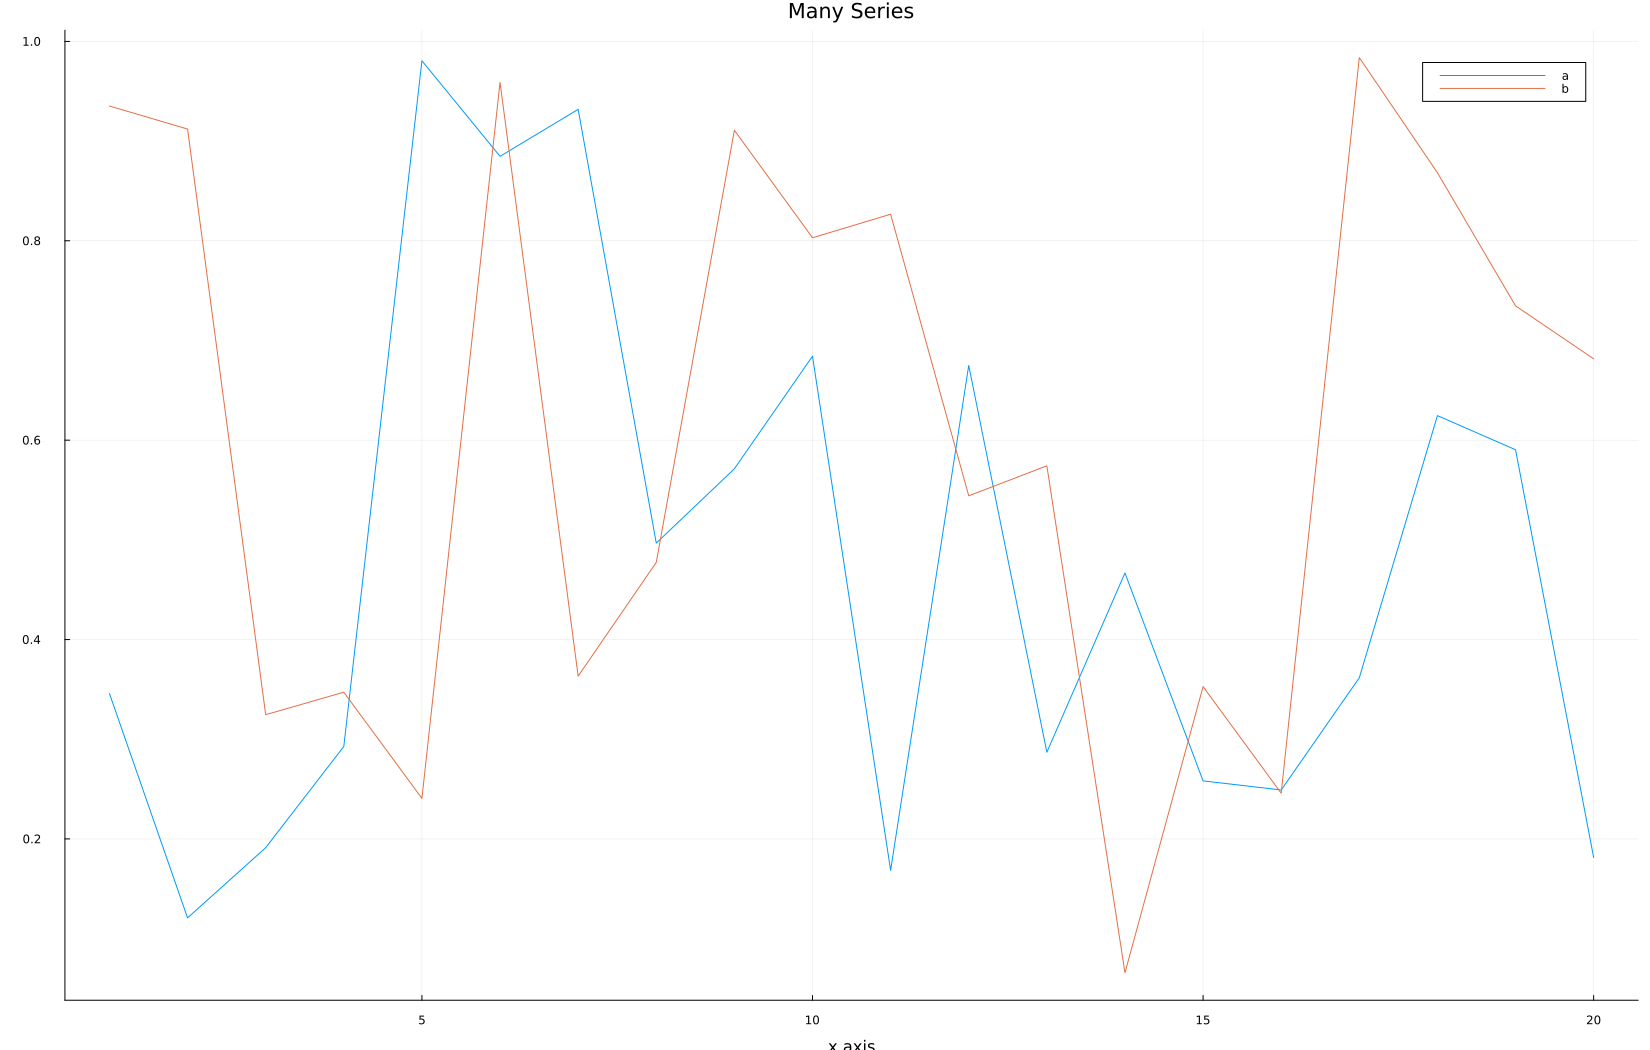
\includegraphics[keepaspectratio]{tutorial-03-05-Plotting_files/mediabag/tutorial-03-05-Plotting_files/figure-pdf/cell-7-output-1.pdf}}

\section{Exercise 2.1 - Customize a Line
Plot}\label{exercise-2.1---customize-a-line-plot}

Now it's your turn to get creative! Customize a line plot with your
choice of colors, line styles, and markers. Save your masterpiece in the
variable \texttt{custom\_line\_plot}.

\begin{Shaded}
\begin{Highlighting}[]
\CommentTok{\# YOUR CODE BELOW}
\CommentTok{\# Hint: Try different line styles (:dash, :dot), colors (:blue, :green), and markers (:star, :diamond)}
\end{Highlighting}
\end{Shaded}

\begin{Shaded}
\begin{Highlighting}[]
\CommentTok{\# Test your answer}
\PreprocessorTok{@assert} \PreprocessorTok{@isdefined}\NormalTok{ custom\_line\_plot}
\FunctionTok{println}\NormalTok{(}\StringTok{"Excellent! You\textquotesingle{}ve created a custom line plot."}\NormalTok{)}
\end{Highlighting}
\end{Shaded}

\begin{tcolorbox}[enhanced jigsaw, colback=white, left=2mm, title=\textcolor{quarto-callout-note-color}{\faInfo}\hspace{0.5em}{Note}, toprule=.15mm, opacitybacktitle=0.6, bottomtitle=1mm, leftrule=.75mm, coltitle=black, breakable, toptitle=1mm, opacityback=0, arc=.35mm, colbacktitle=quarto-callout-note-color!10!white, colframe=quarto-callout-note-color-frame, rightrule=.15mm, bottomrule=.15mm, titlerule=0mm]

Feel free to experiment with different options. There's no ``right''
answer here -- it's all about what looks good to you!

\end{tcolorbox}

\chapter{Section 3 - Adding Multiple Series to a
Plot}\label{section-3---adding-multiple-series-to-a-plot}

Now, let's learn how to add multiple data series to a single plot:

\begin{Shaded}
\begin{Highlighting}[]
\NormalTok{x }\OperatorTok{=} \FloatTok{1}\OperatorTok{:}\FloatTok{20}
\NormalTok{a }\OperatorTok{=} \FunctionTok{rand}\NormalTok{(}\FloatTok{20}\NormalTok{)}
\NormalTok{b }\OperatorTok{=} \FunctionTok{rand}\NormalTok{(}\FloatTok{20}\NormalTok{)}

\NormalTok{multi\_plot }\OperatorTok{=} \FunctionTok{plot}\NormalTok{(}
\NormalTok{    x, a, }
\NormalTok{    title}\OperatorTok{=}\StringTok{"Plot with Two Series"}\NormalTok{, }
\NormalTok{    xlabel}\OperatorTok{=}\StringTok{"X{-}axis"}\NormalTok{, }
\NormalTok{    ylabel}\OperatorTok{=}\StringTok{"Y{-}axis"}\NormalTok{, }
\NormalTok{    label}\OperatorTok{=}\StringTok{"Series A"}
\NormalTok{)}
\FunctionTok{plot!}\NormalTok{(multi\_plot, }
\NormalTok{    x, b, }
\NormalTok{    label}\OperatorTok{=}\StringTok{"Series B"}
\NormalTok{)}

\FunctionTok{display}\NormalTok{(multi\_plot)}
\end{Highlighting}
\end{Shaded}

\pandocbounded{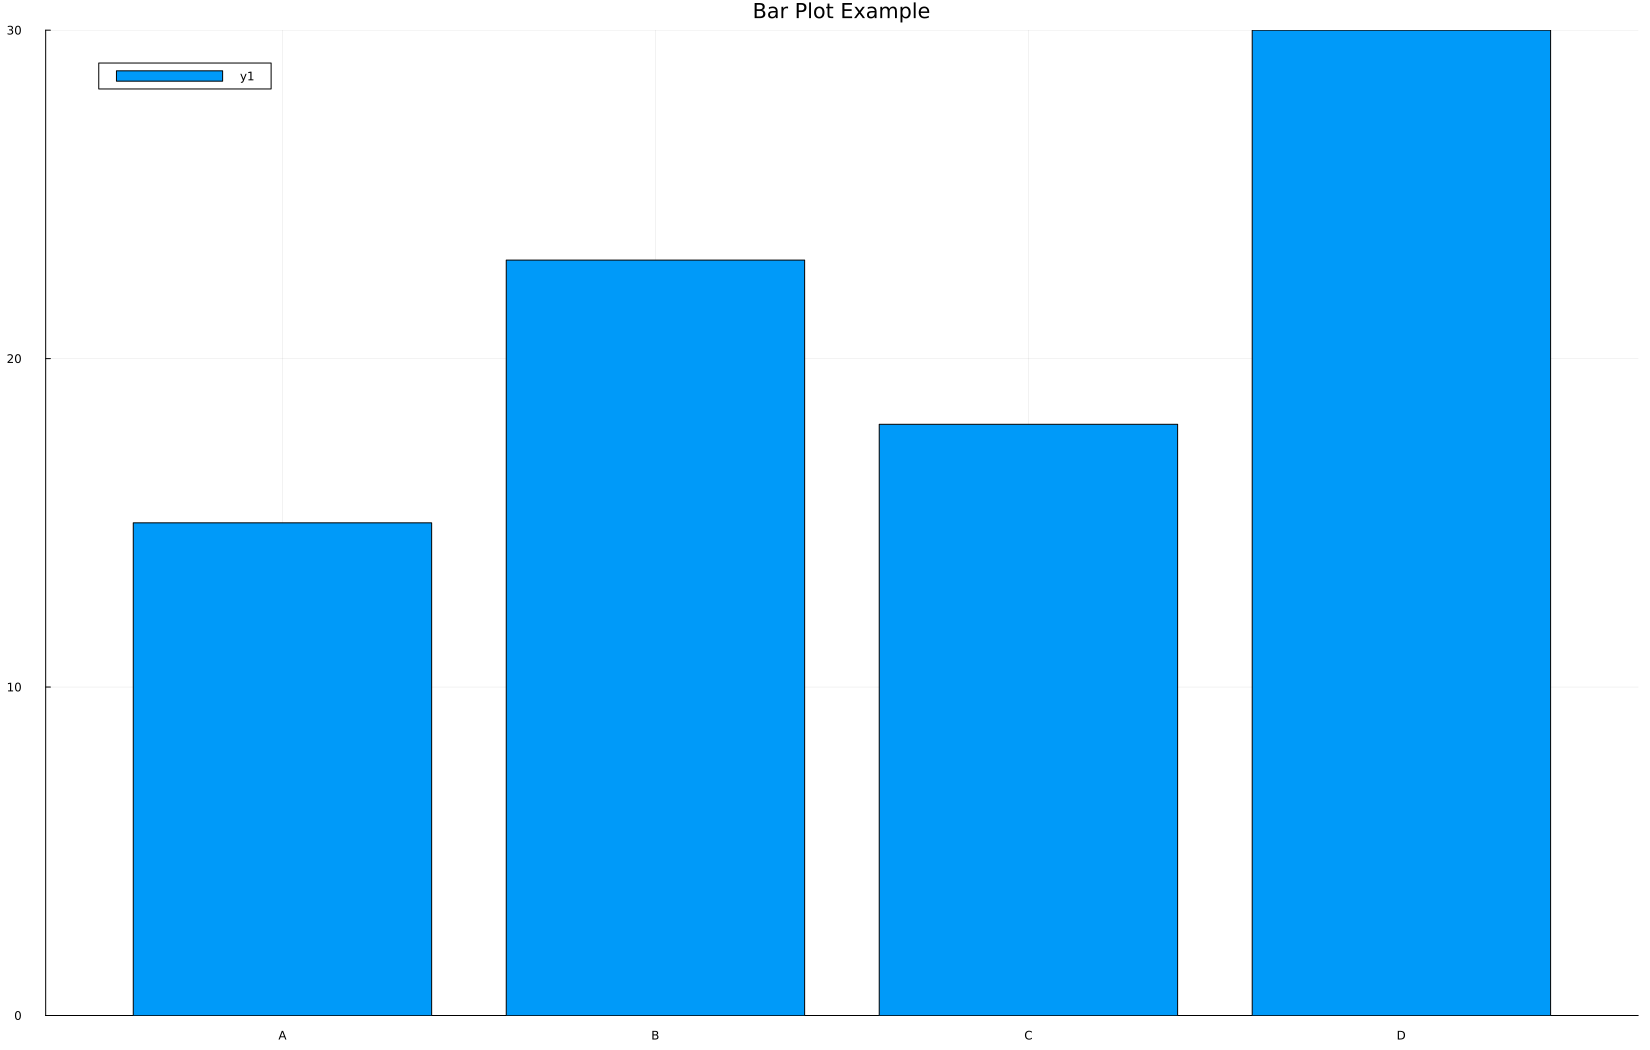
\includegraphics[keepaspectratio]{tutorial-03-05-Plotting_files/mediabag/tutorial-03-05-Plotting_files/figure-pdf/cell-10-output-1.pdf}}

\begin{tcolorbox}[enhanced jigsaw, colback=white, left=2mm, title=\textcolor{quarto-callout-note-color}{\faInfo}\hspace{0.5em}{Note}, toprule=.15mm, opacitybacktitle=0.6, bottomtitle=1mm, leftrule=.75mm, coltitle=black, breakable, toptitle=1mm, opacityback=0, arc=.35mm, colbacktitle=quarto-callout-note-color!10!white, colframe=quarto-callout-note-color-frame, rightrule=.15mm, bottomrule=.15mm, titlerule=0mm]

The \texttt{plot!()} function (with an exclamation mark) adds to an
existing plot instead of creating a new one. In addition, we used the
label here to add a legend to the plot.

\end{tcolorbox}

\section{Exercise 3.1 - Create a Multiple Series
Plot}\label{exercise-3.1---create-a-multiple-series-plot}

NYour turn! Create a plot called \texttt{multi\_series\_plot} with three
data series \texttt{y1}, \texttt{y2}, and \texttt{y3}. Make sure to give
each series a different color and label.

\begin{Shaded}
\begin{Highlighting}[]
\CommentTok{\# YOUR CODE BELOW}
\CommentTok{\# Hint: Use plot() for the first series, then plot!() for the second and third}
\end{Highlighting}
\end{Shaded}

\begin{Shaded}
\begin{Highlighting}[]
\CommentTok{\# Test your answer}
\PreprocessorTok{@assert} \PreprocessorTok{@isdefined}\NormalTok{ y1}
\PreprocessorTok{@assert} \PreprocessorTok{@isdefined}\NormalTok{ y2}
\PreprocessorTok{@assert} \PreprocessorTok{@isdefined}\NormalTok{ y3}
\PreprocessorTok{@assert} \PreprocessorTok{@isdefined}\NormalTok{ multi\_series\_plot}
\FunctionTok{println}\NormalTok{(}\StringTok{"Fantastic! You\textquotesingle{}ve created a plot with multiple series."}\NormalTok{)}
\end{Highlighting}
\end{Shaded}

\chapter{Section 3 - Saving Plots to
Files}\label{section-3---saving-plots-to-files}

Plots.jl supports saving your plots to various file formats including
PNG, SVG, and PDF, enabling you to use your plots outside of Julia. The
function to save plots is \texttt{savefig()}, the first argument is the
plot itself and the second argument is the \texttt{path/filename} format
as string. Replace \texttt{path} with the path, the \texttt{filename}
with the actual name and \texttt{format} with the file format,
e.g.~\texttt{pdf}, \texttt{png}, \ldots{} . For example, if you want to
save your file as PDF, you would just name it
\texttt{path/filename.pdf}. For example:

\begin{Shaded}
\begin{Highlighting}[]
\FunctionTok{savefig}\NormalTok{(plot\_name, }\StringTok{"path/filename.png"}\NormalTok{)}
\end{Highlighting}
\end{Shaded}

This saves the plot as a PNG file.

\section{Exercise 3.1 - Save a Plot to a
File}\label{exercise-3.1---save-a-plot-to-a-file}

Save your \texttt{multi\_series\_plot} as a PNG file named
``saved\_plot.png'' in the ``ExampleData'' folder.

\begin{Shaded}
\begin{Highlighting}[]
\CommentTok{\# YOUR CODE BELOW}
\CommentTok{\# Don\textquotesingle{}t forget to use the @\_\_DIR\_\_ macro to get the correct file path!}
\end{Highlighting}
\end{Shaded}

\begin{Shaded}
\begin{Highlighting}[]
\CommentTok{\# Test your answer}
\PreprocessorTok{@assert} \FunctionTok{isfile}\NormalTok{(}\StringTok{"}\SpecialCharTok{$}\NormalTok{(}\PreprocessorTok{@\_\_DIR\_\_}\NormalTok{)}\StringTok{/ExampleData/saved\_plot.png"}\NormalTok{) }\StringTok{"File does not exist yet."}
\FunctionTok{println}\NormalTok{(}\StringTok{"Well done! You\textquotesingle{}ve saved your plot as an image file."}\NormalTok{)}
\end{Highlighting}
\end{Shaded}

\chapter{Section 4 - Advanced Plotting
Techniques}\label{section-4---advanced-plotting-techniques}

Let's explore some other common plot types. While you don't have to
solve any task here, the code might come in handy later on during the
course as recipe.

\section{Bar Plot}\label{bar-plot}

\begin{Shaded}
\begin{Highlighting}[]
\CommentTok{\# Bar plot}
\NormalTok{x\_categories }\OperatorTok{=}\NormalTok{ [}\StringTok{"A"}\NormalTok{, }\StringTok{"B"}\NormalTok{, }\StringTok{"C"}\NormalTok{, }\StringTok{"D"}\NormalTok{]}
\NormalTok{y\_values }\OperatorTok{=}\NormalTok{ [}\FloatTok{15}\NormalTok{, }\FloatTok{23}\NormalTok{, }\FloatTok{18}\NormalTok{, }\FloatTok{30}\NormalTok{]}
\NormalTok{bar\_plot }\OperatorTok{=} \FunctionTok{bar}\NormalTok{(}
\NormalTok{    x\_categories, }
\NormalTok{    y\_values, }
\NormalTok{    title}\OperatorTok{=}\StringTok{"Bar Plot Example"}
\NormalTok{)}
\FunctionTok{display}\NormalTok{(bar\_plot)}
\end{Highlighting}
\end{Shaded}

\pandocbounded{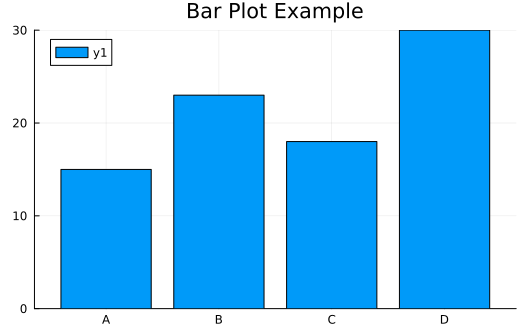
\includegraphics[keepaspectratio]{tutorial-03-05-Plotting_files/mediabag/tutorial-03-05-Plotting_files/figure-pdf/cell-15-output-1.pdf}}

\section{Histogram}\label{histogram}

\begin{Shaded}
\begin{Highlighting}[]
\NormalTok{data }\OperatorTok{=} \FunctionTok{randn}\NormalTok{(}\FloatTok{1000}\NormalTok{)}
\NormalTok{hist\_plot }\OperatorTok{=} \FunctionTok{histogram}\NormalTok{(}
\NormalTok{    data, }
\NormalTok{    bins}\OperatorTok{=}\FloatTok{30}\NormalTok{, }
\NormalTok{    title}\OperatorTok{=}\StringTok{"Histogram Example"}
\NormalTok{)}
\FunctionTok{display}\NormalTok{(hist\_plot)}
\end{Highlighting}
\end{Shaded}

\pandocbounded{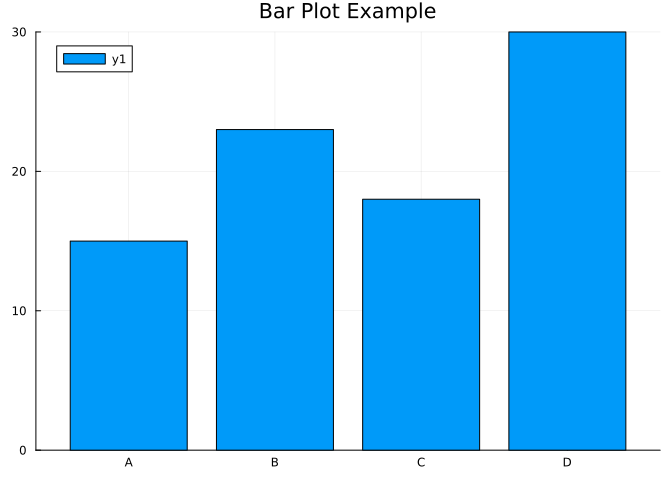
\includegraphics[keepaspectratio]{tutorial-03-05-Plotting_files/mediabag/tutorial-03-05-Plotting_files/figure-pdf/cell-16-output-1.pdf}}

\section{Box Plot}\label{box-plot}

\begin{Shaded}
\begin{Highlighting}[]
\CommentTok{\# Box plot}
\NormalTok{group }\OperatorTok{=} \FunctionTok{repeat}\NormalTok{(}\FloatTok{1}\OperatorTok{:}\FloatTok{4}\NormalTok{, inner}\OperatorTok{=}\FloatTok{50}\NormalTok{)}
\NormalTok{y }\OperatorTok{=} \FunctionTok{randn}\NormalTok{(}\FloatTok{200}\NormalTok{) }\OperatorTok{.+}\NormalTok{ group}
\NormalTok{box\_plot }\OperatorTok{=} \FunctionTok{boxplot}\NormalTok{(}
\NormalTok{    group, }
\NormalTok{    y, }
\NormalTok{    title}\OperatorTok{=}\StringTok{"Box Plot Example"}
\NormalTok{)}
\FunctionTok{display}\NormalTok{(box\_plot)}
\end{Highlighting}
\end{Shaded}

\pandocbounded{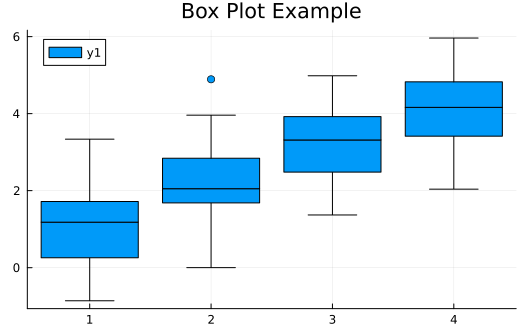
\includegraphics[keepaspectratio]{tutorial-03-05-Plotting_files/mediabag/tutorial-03-05-Plotting_files/figure-pdf/cell-17-output-1.pdf}}

\chapter{Conclusion}\label{conclusion}

Fantastic! You've completed the tutorial on basic plotting in Julia.
You've learned how to create basic plots and customize and save them.
Continue to the next file to learn more.

\chapter{Solutions}\label{solutions}

You will likely find solutions to most exercises online. However, I
strongly encourage you to work on these exercises independently without
searching explicitly for the exact answers to the exercises.
Understanding someone else's solution is very different from developing
your own. Use the lecture notes and try to solve the exercises on your
own. This approach will significantly enhance your learning and
problem-solving skills.

Remember, the goal is not just to complete the exercises, but to
understand the concepts and improve your programming abilities. If you
encounter difficulties, review the lecture materials, experiment with
different approaches, and don't hesitate to ask for clarification during
class discussions.

Later, you will find the solutions to these exercises online in the
associated GitHub repository, but we will also quickly go over them in
next week's tutorial. To access the solutions, click on the Github
button on the lower right and search for the folder with today's lecture
and tutorial. Alternatively, you can ask ChatGPT or Claude to explain
them to you. But please remember, the goal is not just to complete the
exercises, but to understand the concepts and improve your programming
abilities.




\end{document}
